\lstset{
  basicstyle=\ttfamily,
  columns=fullflexible,
  frame=single,
  breaklines=true,
  postbreak=\mbox{\textcolor{red}{$\hookrightarrow$}\space},
}

\subsection{Shutter Timing issue}
Since the first photon observation was made, the shutter system has exhibited issues including the blade overran, leaving the hsutter partially opened, and discontinuities in motion profiles \citep{CTN-003}. This section presents the further analysis and results of follow-up tests, and current understanding and remaining open questions.

\subsubsection{Overview of the shutter operation}
The camera shutter is controlled by the Beckhoff TwinCAT PLC system. The CCS sends commands to a Beckhoff CX5120 controller, which is an industrial PC running Windows 7 Embedded Standard along with a real-time kernel called TwinCAT 3. This is the gateway and manages the PLC system interconnected by EtherCAT. The PLC system consists of various "terminal" modules that can take different roles, such as controlling digital and analog I/O as well as the timing module, so-called EL6688. EL6688 provides an external reference to synchronize the clock among terminals with the GPS clock in a better accuracy than 1$\mu$s. 

In this system, there are concepts of 4 different clocks: 
\begin{enumerate}
    \item The CCS clock synchronized by NTP, which is based on UTC,
    \item The TwinCAT Windows clock, which is supposed to be synchronized by NTP and should have been identical to (1); however, the chrony (NTP) service on the gateway machine of the shutter system has not been configured to provide the clock to the Beckhoff Windows \href{https://rubinobs.atlassian.net/browse/LSSTCAM-146}{LSSTCAM-146}
    \item Distributed clock (DC) in the TwinCAT PLC system. When the shutter blade passes the hole sensors placed along with the shutter rail, the PLC is programmed to trigger the timing measurement based on DC. This timing information is the foundation of the motion profile as well as the entire timing control of the PLC system.
    \item External reference clock from EL6688. The time source is a GPS clock in the observatory and the synchronization is provided by Precisioon Timing Protocol, which is expected to provide sub-microsecond timing accuracy through network delay measurements.
\end{enumerate}

\begin{figure}
    \centering
    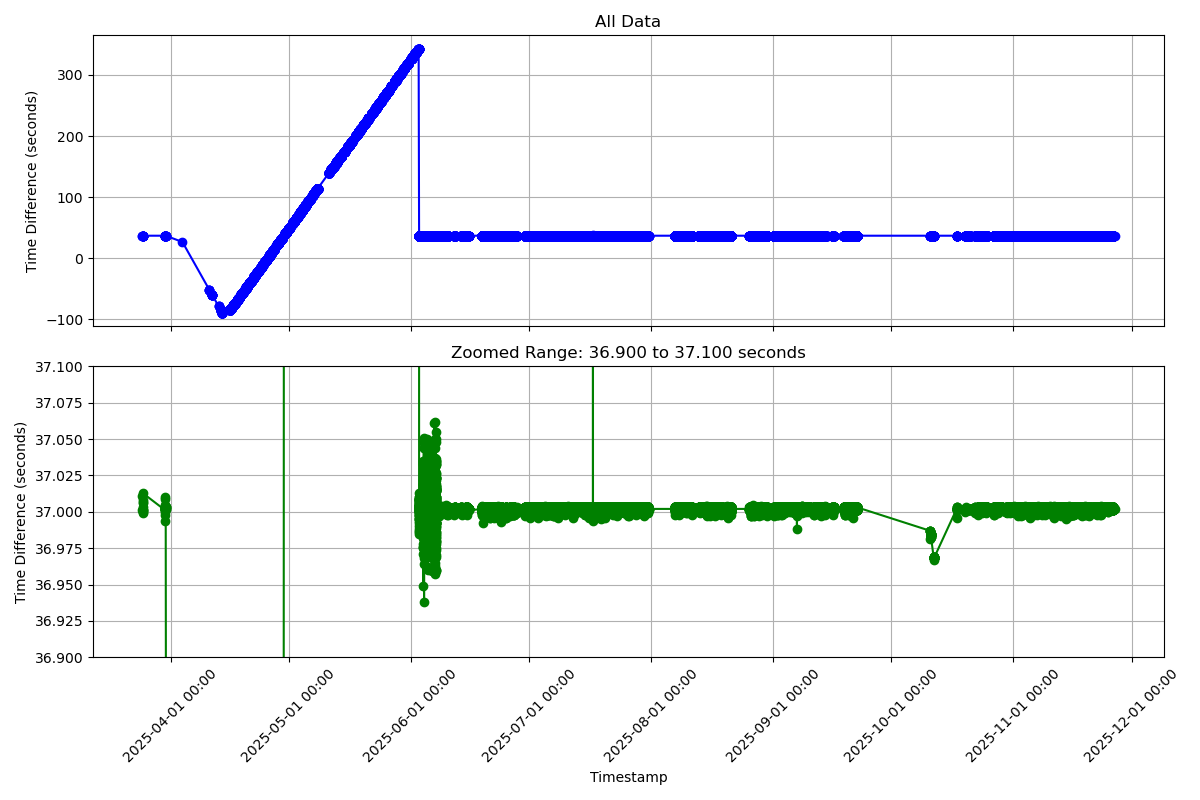
\includegraphics[width=1.0\linewidth]{shutter/time_diff_two_panel.png}
    \caption{Timing between the CCS time when takeExposure was recorded and the time when the motion profile records the startTime. This doesn't reflect the actual shutter motion timing.}
    \label{fig:shutterclocks}
\end{figure}
We investigate the consistency in the timings from logging messages retroactively. The focus is given on the CCS clock and the DC time reported by the motion profile. The UTC timestamps in the MCM log (`sent takeExposure to shutter1'') were paired with TAI timestamps from motion profiles (`startTime.tai.isot''). Because TAI leads UTC by 37 seconds, the expected difference is approximately: \textit{37 seconds + system/network jitter.}
Plotting these deltas revealed three operational periods in Figure \ref{fig:shutterclocks}.  There are three distinct periods in this plot.

\textit{April--June 2:} The EL6688 was intermittently synchronized (the reported PTP state was unstable, bouncing between LISTENING (4) and SLAVE (9) states). However, evidence suggests that DC time was free-running. The shutter became unstable near the end of this period, including discontinuities in the motion profiles and blade overrun issues. This period ended after power was initialized to the shutter system. The underlying cause remains unknown.  A reduction in TCPSynRetrans was observed, which may indicate a Linux kernel–level anomaly. 

\textit{June 3--June 7:} The EL6688 synchronized to a MOXA boundary clock, but synchronization quality was poor. Observed scatter reached 50 ms. The MOXA switch is an internal L2 network switch inside the Camera (EDS-G516E-T). As described in \citet{CTN-003}, the PTP functionality of the MOXA switch does not appear to function correctly with the observatory network. The communication with the vendor confirmed that this device only supports the software-based PTP and does not support the hardware-based PTP which can explain the poor quality of the synchronization. 

\textit{June 8--Dec 2 (present):} The EL6688 synchronized to an observatory boundary clock on a leaf switch (10.17.200.33) after three hops from the Grand Master Clock, where the GPS clock is connected. Timing has remained stable.

\subsubsection{Verification of the Observatory's PTP}
% verification of the observatory's PTP system
Further analysis was conducted using the spare system lsstcam-shutter02 in the clean room. This system is connected to the observatory's network. This network is specially configured to pass the PTP packets. The network routes through an identical MOXA switch, providing an opportunity to investigate whether the observatory's PTP system functions as intended and to identify any issues with the MOXA switch. Tests conducted in the clean room revealed successful PTP synchronization using a MOXA operating as an L2 switch by the following command:


\begin{lstlisting}
[yutsumi@lsstcam-shutter02 ~]$  sudo ptp4l -f /etc/ptp4l.conf -i enp0s31f6 -m
[sudo] password for yutsumi: 
ptp4l[503690.709]: selected /dev/ptp1 as PTP clock
ptp4l[503690.710]: port 1 (enp0s31f6): INITIALIZING to LISTENING on INIT_COMPLETE
ptp4l[503690.710]: port 0 (/var/run/ptp4l): INITIALIZING to LISTENING on INIT_COMPLETE
ptp4l[503690.710]: port 0 (/var/run/ptp4lro): INITIALIZING to LISTENING on INIT_COMPLETE
ptp4l[503696.415]: port 1 (enp0s31f6): new foreign master fc59c0.ffff.214803-29
ptp4l[503712.418]: selected best master clock 000efe.fffe.011598
ptp4l[503712.418]: port 1 (enp0s31f6): LISTENING to UNCALIBRATED on RS_SLAVE
ptp4l[503714.237]: port 1 (enp0s31f6): minimum delay request interval 2^5
ptp4l[503714.620]: master offset -311009524 s0 freq   +6354 path delay     10727
ptp4l[503715.623]: master offset -311010780 s1 freq   +5099 path delay     10727
ptp4l[503716.621]: master offset        474 s2 freq   +5573 path delay     10727
ptp4l[503716.621]: port 1 (enp0s31f6): UNCALIBRATED to SLAVE on MASTER_CLOCK_SELECTED
ptp4l[503717.623]: master offset       1484 s2 freq   +6725 path delay     10727
ptp4l[503718.625]: master offset        257 s2 freq   +5943 path delay     10727
ptp4l[503719.623]: master offset        -26 s2 freq   +5737 path delay     10727
ptp4l[503720.628]: master offset       -184 s2 freq   +5571 path delay     10727
ptp4l[503721.626]: master offset          8 s2 freq   +5708 path delay     10727
ptp4l[503722.626]: master offset        443 s2 freq   +6145 path delay     10727
ptp4l[503723.631]: master offset         83 s2 freq   +5918 path delay     10727
ptp4l[503724.631]: master offset       -434 s2 freq   +5426 path delay     10727
ptp4l[503725.635]: master offset       -149 s2 freq   +5581 path delay     10727
\end{lstlisting}
The offset is in nanoseconds unit and s2 indicates the servo is in the locked state. As indicated in the output, the offset converges quickly. The key in the configuration is that the priorities have to be 255 since the priority of the grandmaster is set to be 255, otherwise lsstcam-shutter takes the grandmaster role in the PTP system which screws up the PTP synchronization.
These tests confirm the observatory's PTP functionality.

There is another machine in the clean room Dell AIO, aio06. This machine was also used to test the PTP. The hardware clock behaved poorly under frequency adjustment, but acceptable synchronization was achieved using weakened servo parameters:
\begin{lstlisting}
[lsstcam-aio06] % sudo ptp4l -f /etc/ptp4l.conf -i enp0s31f6 -m -H  --step_threshold=1  --pi_proportional_const=0.01  --pi_integral_const=0.0001
\end{lstlisting}

% verification of the EL6688:`
\subsubsection{Verification with the spare shutter system}
Since the PTP synchronization has been successfully established with linux computers through the MOXA switch, the focus moves onto the actual PTP terminal module EL6688.  EL6688 was particullary difficult because the interface only supports 100Mbps connection. There was a doubt whether the link speed conversion does not interfere with the PTP synchronization. We used several tools to investigate the PTP synchronization comprehensively.

`readPtpDiag.sh` is the tool to communicates with Beckhoff controller over the network, which provides a partial view of the variables in the PLC. The following example is taken from \cite{CTN-003}.
\begin{lstlisting}
[ccs@lsstcam-shutter02 ~]$ /usr/local/bin/readPtpDiag.sh 
HCU date and time:           2025-06-09 17:58:35.614918
PTP version:                 PTPv2 (32)
PTP state:                   SLAVE (9)
Clock ID (hex):              00 01 05 ff fe 3e 4c 43
Master clock ID (hex):       fc 59 c0 ff ff 21 48 03 00 1d
Grandmaster clock ID (hex):  00 0e fe ff fe 01 15 98
Offset from master (ns):     -11,662
Mean path delay (ns):        122,992
Steps removed:               4
Sync msg sequence no.:       37388
Time scale:                  PTP/TAI (1)
Offset from UTC (sec):       37
UTC offset valid?            True
Leap61?                      False
Leap59?                      False
Epoch no.:                   0
External (PTP) time:         Wed, 16 Jul 2025 17:40:44.907797 UTC
\end{lstlisting}
The output has a few distinct states every power cycle. "Offset from Master" is sometimes quite large, as large as $10^9$ nanoseconds (or 1 second), and sometimes it is small as an order of 10$\mu$s or could be smaller, regardless of the "PTP state". And sometimes the PTP state never becomes SLAvE(9) but LISTENING(4).


Windows's program TwinCAT XAE shell (TcXaeShell) provides a live and full view of the variables in the PLC system. Figure \ref{fig:TcXaeShell} shows an example screenshot of TcXaeShell when the vendor-provided example project is running. DcToTcTimeOffset and DcToExtTimeOffset are one of the important variables because we found that they tell which of either TwinCAT or PTP clock is used to synchronize to DC. It appears that only one of them becomes non-zero, and the other becomes zero but randomly. Whether which clock is used is not deterministic as long as we use TwinCAT version 3.14022.36.

bSynchronized and nTimeDiff are also important parameters. These are unique in the vendor-provided project. These tell us whether EL6688 is synchronized with PTP or not and how much delay is observed. The meaning of the synchronization in the vendor implementation is broad. The synchronization is established regardless of whether the DC is synchronized to the Beckhoff Windows or EL6688, since EL6688 gives a reference clock and the actual clock synchronization is done in the Beckhoff Windows system using  \href{https://confluence.slac.stanford.edu/spaces/LSSTCAM/pages/246939969/PTP+module+EL6688+for+the+Beckhoff+controller#PTPmoduleEL6688fortheBeckhoffcontroller-HowtoconvertDCtimetoTAI64Ntime}{the built-in functions}. nTimeDiff seems to be different from Offset from master. 
\begin{figure}
    \centering
    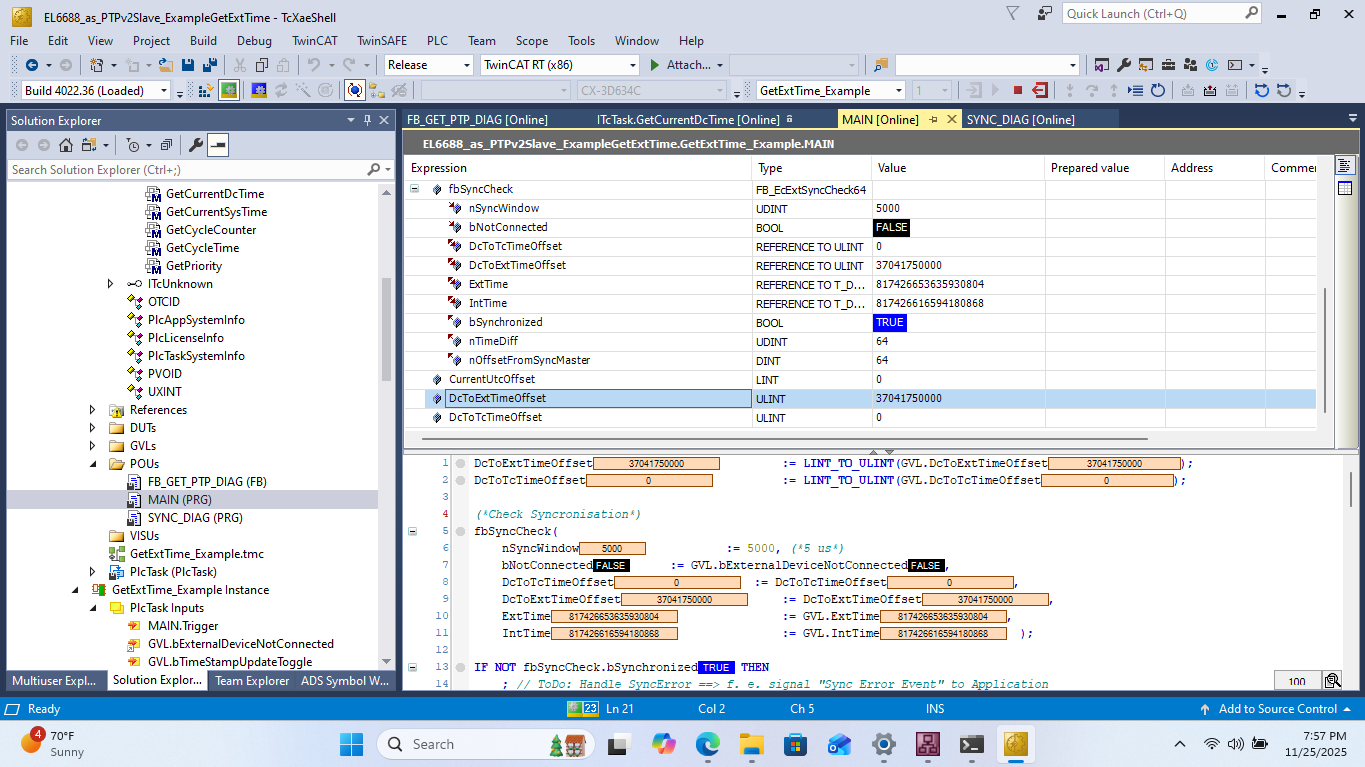
\includegraphics[width=\linewidth]{shutter/ScreenshotOfSample.png}
    \caption{A screenshot of the vendor provided sample program. DcToTcTimeOffset, DcToExtTimeOffset and bSynchronized as well as nTimeDiff are displayed in this screenshot.}
    \label{fig:TcXaeShell}
\end{figure}

Another diagnostic tools is a generic open-source software, tcpdump.
\begin{verbatim}
    sudo tcpdump -i enp0s31f6 -n -s 0 'ether proto 0x88f7 or udp port 319 or udp port 320' -a
\end{verbatim}
The example output of tcpdump is the following, focusing on a communication pair between the boundary clock and the client (EL6688) when they exchange "delay request" and "delay response".
\begin{lstlisting}
12:33:01.777635 IP 139.229.175.116.ptp-event > 224.0.1.129.ptp-event: PTPv2, v1 compat : no, msg type : delay req msg, length : 44, domain : 0, reserved1 : 0, Flags [none], NS correction : 0, sub NS correction : 0, reserved2 : 0, clock identity : 0x105fffe3e4c43, port id : 1, seq id : 8038, control : 1 (delay req msg), log message interval : 5, originTimeStamp : 1764419582 seconds, 136332373 nanoseconds
12:33:01.777892 IP 10.17.200.33.ptp-general > 224.0.1.129.ptp-general: PTPv2, v1 compat : no, msg type : delay resp msg, length : 54, domain : 0, reserved1 : 0, Flags [none], NS correction : 0, sub NS correction : 0, reserved2 : 0, clock identity : 0xfc59c0ffff214803, port id : 29, seq id : 8038, control : 3 (peer delay resp msg), log message interval : 5, receiveTimeStamp : 1764419618 seconds, 777492282 nanoseconds, port identity : 0x105fffe3e4c43, port id : 1
\end{lstlisting}
This example confirms that EL6688 communicates with the boundary clock (a leaf switch) directly, regardless of the presence of the MOXA L2 switch. This message exchange is a part of the foundation to measure the delay in the communication, which enables precise timing synchronization as defined in the PTP specification. In this case, the time difference from originTimeStamp to receiveTimeStamp is 36.641159909 sec. Repeating observations of these packets found that delays are consistent over multiple days with a better accuracy than 1$\mu$s.

Although the difference is consistent, the difference itself is quite large. This large difference was observed when the large Offset from master was observed (DC is synchronized with the TwinCAT clock). On the other hand, if DC is synchronized with EL6688/PTP, the difference was quite small. This observation suggests that when the DC synchronized with the TwinCAT clock and the DC tries to keep the pace as referenced from EL6688 (PTP) but likely the absolute clock could be wrong if TWinCAT clock is not reasonably synchronized with NTP.

\subsubsection{Summary}\
\begin{itemize}
\item The observatory PTP system provides a reasonable PTP sychronization.
\item MOXA switch does not support the hardware clock, resutling in the poor PTP synchronization. 
\item Even EL6688 supports up to 100Mbps, reasonable synchronization can be established.
\item TwinCAT's behavior whether DC is synchronized to TwinCAT controller or EL6688 is not consistent and not configurable. Power cycle until it has a small enough offset from Master is needed operationally.
\item {\bf We also note that motion profile timing prior to June 7 should be considered unreliable; afterward, it appears trustworthy.} 
\item The jumps in the motion profile can be explained by intermittent adjustment based on the EL6688 to the TwinCAT system appears to play a role here. 
\end{itemize}

\textbf{Recommendations}\
\begin{itemize}
\item Correct the Puppet-managed chrony.conf on shutter01/shutter02 (\href{https://rubinobs.atlassian.net/browse/LSSTCAM-146}{LSSTCAM-146}).
\item Perform the Chris Walter timing test to interdependently check the timing accuracy. \cite{SITCOMTN-136}
\item Consider to increase the proprieties (lower the number) of the observatory grandmaster/boundary clocks. Any misconfigured computer can mess up the PTP network as ptp4l's default is 128.
\end{itemize}

 
\textbf{Open Questions}\
\begin{itemize}
\item Beckhoff's statement that EL6688 ``does not adjust the distributed clock'' remains unclear, especially regarding NTP/PTP coexistence.
\item Compare MCM command timestamps with motion profile timestamps for deeper latency characterization.
\item Determine whether shutter02 can store/export motion profiles for analysis.
\end{itemize}

